\documentclass[useAMS,usenatbib]{mn2e}
\usepackage{footnote}
\usepackage{graphicx}
\usepackage{amsmath}
\usepackage{natbib}
\usepackage{array}
\usepackage{color}
\usepackage{url}
\usepackage{multirow}
\voffset=-0.5in
\pdfminorversion=5
\setlength{\parsep}{0pt}
\setlength{\partopsep}{0pt}
\def\starpy {\textsc{starpy}}


\begin{document}

\title[]{Bayesian methods for determining galactic star formation histories}
\author[Smethurst 2015]{R. ~J. ~Smethurst,$^{1}$
\\ $^1$ Oxford Astrophysics, Department of Physics, University of Oxford, Denys Wilkinson Building, Keble Road, Oxford, OX1 3RH, UK }

\maketitle

\begin{abstract}

Does galaxy evolution proceed across the colour magnitude diagram via multiple pathways or as a single population? For my thesis I have attempted to answer this general question through the use of a new Bayesian determination of the most likely star formation history of a galaxy given it's observed optical and NUV photometry. Using this new method and classifications from Galaxy Zoo I have been able to show that diverse morphologically dependant quenching mechanisms with a range of quenching rates are all instrumental in the formation of the present day red sequence. This is contrary to previous work highlighting radically different evolutionary pathways between early- and late-type galaxies. I have extended this work to explore the relationship between these quenched star formation histories and the presence of a type 2 AGN, finding evidence to show that a population of these AGN host galaxies have recently undergone a rapid drop in their star formation rate. This result provides strong observational support for AGN feedback in these systems, but this work also shows that feedback cannot be responsible for all of the quenching across the AGN host population. I shall discuss these results and how they will contribute to my thesis. 

\end{abstract}

\section{Introduction}

Previous large scale surveys of galaxies have revealed a bimodality in the colour-magnitude diagram (CMD) with two distinct populations; one at relatively low mass, with blue optical colours and another at relatively high mass, with red optical colours \citep{Baldry04, Baldry06, Willmer06, BLB08, Brammer09}. These populations were dubbed the `blue cloud' and `red sequence' respectively.

The sparsely populated colour space between these two populations, the so-called `green valley', provides clues to the nature and duration of galaxies' transitions from blue to red. These transitions must occur on rapid timescales, otherwise we would observe an accumulate of galaxies in the green valley. Green valley galaxies are therefore thought to be a transition population between the blue cloud and the `dead' red sequence \citep{Martin07, Faber07, Mendez11, Gonc12}. 

The intermediate colours of these green valley galaxies have been interpreted as evidence for recent quenching (suppression) of star formation \citep{Salim07}. Star forming galaxies are observed to lie on a well defined mass-SFR relation, however quenching a galaxy causes it to depart from this relation (\citealt{Noeske07, Peng}).

By studying the galaxies which  have just left this mass-SFR relation, the quenching mechanisms by which this occurs can be probed. There have been many previous theories for the initial triggers of these quenching mechanisms, including negative feedback from AGN \citep{Sch07}, mergers \citep{Darg10a}, supernovae winds \citep{MFB12} and secular evolution \citep{Masters10, Masters11}. In particular observations of AGN host galaxies reveal their location in the green valley, suggesting a particular role for AGN feedback in the process of quenching \citep{Nandra07, Hasinger08, Silverman08, Sch2014}. By investigating the \emph{amount} of quenching that has occurred across the colour magnitude diagram and in a population of AGN host galaxies, constraints to these quenching mechanism theories can be applied. 

To investigate the rates of quenching and therefore the possible mechanisms I have implemented a simple novel method utilising Bayesian statistics (for a comprehensive overview of Bayesian statistics see either \citealt{MacKay} or \citealt{Sivia}) in order to find the typical model parameters of the star formation history of galaxies in a given population. Previous investigations have only implemented frequentist methods on small sample sizes; however here I have implemented Bayesian methods on large populations of galaxies to determine the evolution. I have assumed the simplest model possible in order to derive any useful information before implementing more sophisticated techniques in future work. 


\section{Methods}

\textsc{starpy}\footnote{Publicly available: \url{http://github.com/zooniverse/starpy}} is a \textsc{python} code which allows the user to derive the quenched star formation history (SFH) of a galaxy through a Bayesian Markov Chain Monte Carlo method \citep{Dan}\footnote{\url{http://dan.iel.fm/emcee/}} with the input of the observed $u-r$ and $NUV-u$ colours, a redshift, and the use of the stellar population models of \cite{BC03}. The star formation history template is an exponential decline of the SFR and is described by two parameters $[t_q, \tau]$, where $t_q$ is the time at which the onset of quenching begins $\rm{[Gyr]}$ and $\tau$ is the exponential rate at which quenching occurs $\rm{[Gyr]}$. Under the simplifying assumption that all galaxies formed at $t=0$ $\rm{ Gyr}$ with an initial burst of star formation, the SFH can be described as: 
\begin{equation}\label{sfh}
SFR =
\begin{cases}
i_{sfr}(t_q) & \text{if } t < t_q \\
i_{sfr}(t_q) \times exp{\left( \frac{-(t-t_{q})}{\tau}\right)} & \text{if } t > t_q 
\end{cases}
\end{equation}
where $i_{sfr}$ is an initial constant star formation rate dependent on $t_q$ \citep{Sch2014, Sme2015}.  A smaller $\tau$ value corresponds to a rapid quench, whereas a larger $\tau$ value corresponds to a slower quench. The output of \starpy  ~ is probabilistic in nature and provides the posterior probability distribution across the entirety of the two parameter space for each individual galaxy. The probabilistic fitting methods to this SFH for an observed galaxy are described in full detail in \cite{Sme2015}. 

We apply this method to derive the quenched SFHs of a sample of $126, 316$ SDSS galaxies also observed with GALEX (to acquire NUV photometry) that have been classified by the Galaxy Zoo 2 project \cite{GZ2}. We refer to this as the \textsc{gz2-galex} sample. The output is a 2-dimensional likelihood distribution across the $[t_q, \tau]$ parameter space for each individual galaxy. We sum individual galaxy likelihood distributions across the blue cloud, green valley and red sequence populations of the colour magnitude diagram, additionally weighting by the GZ2 morphologies to produce quenching parameter likelihood distributions for both disc- and smooth-dominated galaxy populations. 

\section{Results to Date}

\subsection{Quenching across the Colour Magnitude Diagram}\label{gv}

\begin{figure*}
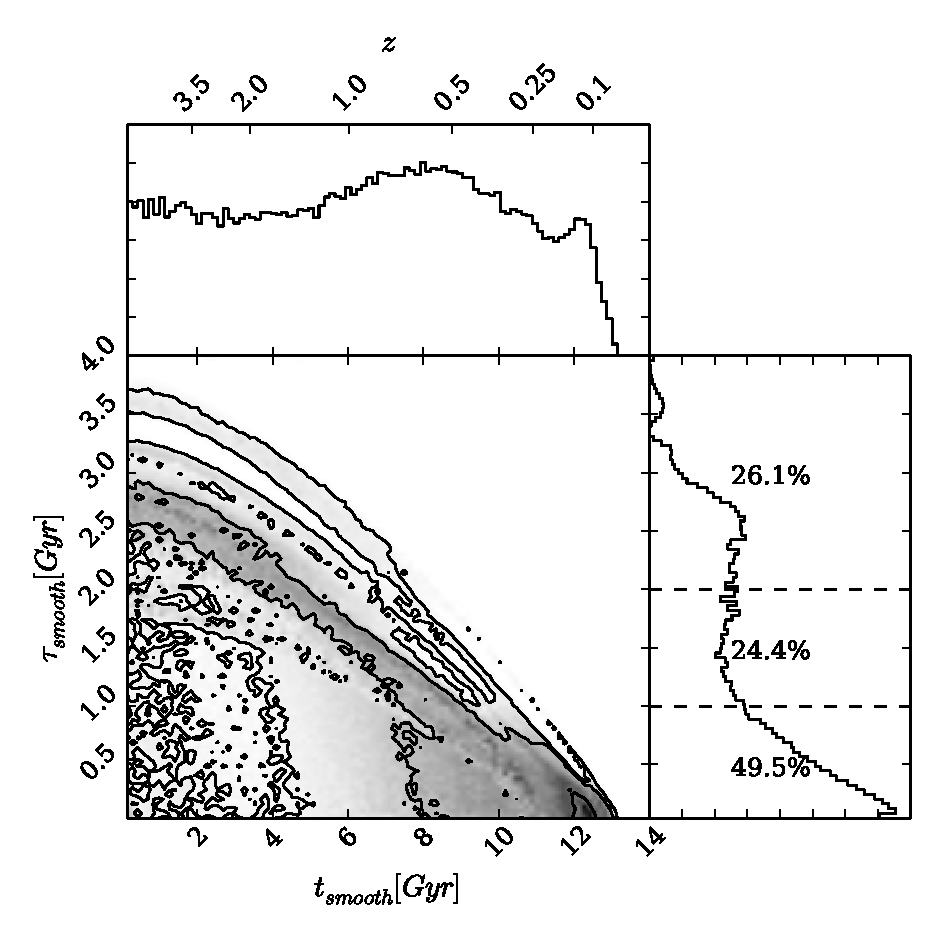
\includegraphics[width=0.4975\textwidth]{red_smooth.pdf}
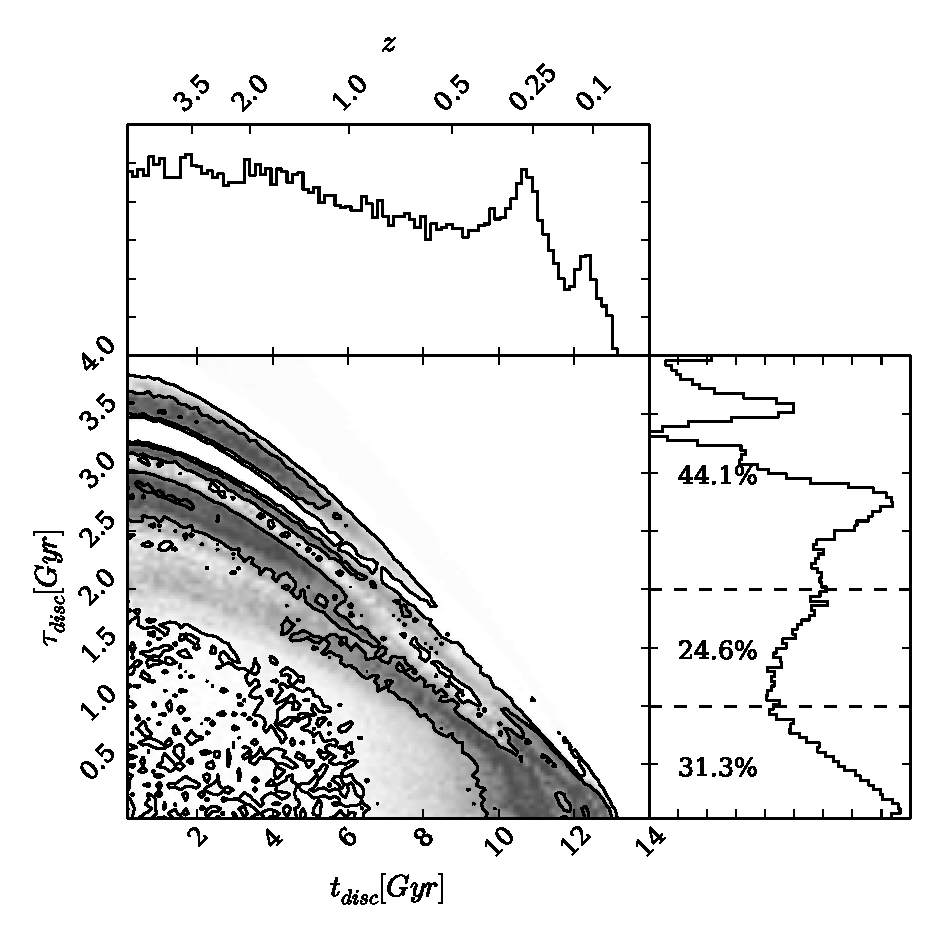
\includegraphics[width=0.4975\textwidth]{red_disc.pdf}
\caption{Contour plots showing the summed posterior probability distribution function weighted by the morphological vote fractions from GZ2 to give the areas of high likelihood in the model parameter space for both elliptical (left) and disc (right) dominated systems. The histograms show the projection into one dimension for each parameter. The dashed lines show the separation between rapid ($\tau ~\rm{[Gyr]} < 1.0$), intermediate ($1.0 < \tau ~\rm{[Gyr]} < 2.0$) and slow ($\tau ~\rm{[Gyr]} > 2.0$) quenching timescales with the fraction of the combined posterior probability distribution in each region shown}.
\label{red_s}
\end{figure*}

\begin{figure*}
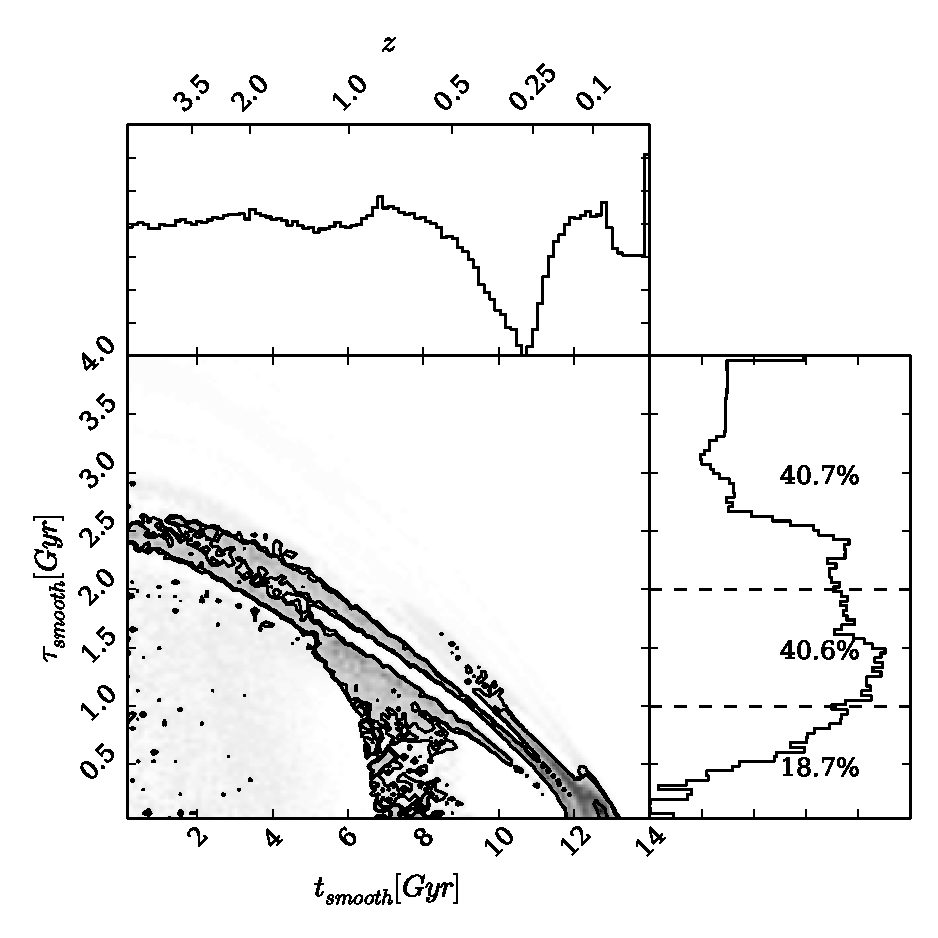
\includegraphics[width=0.4975\textwidth]{green_smooth.pdf}
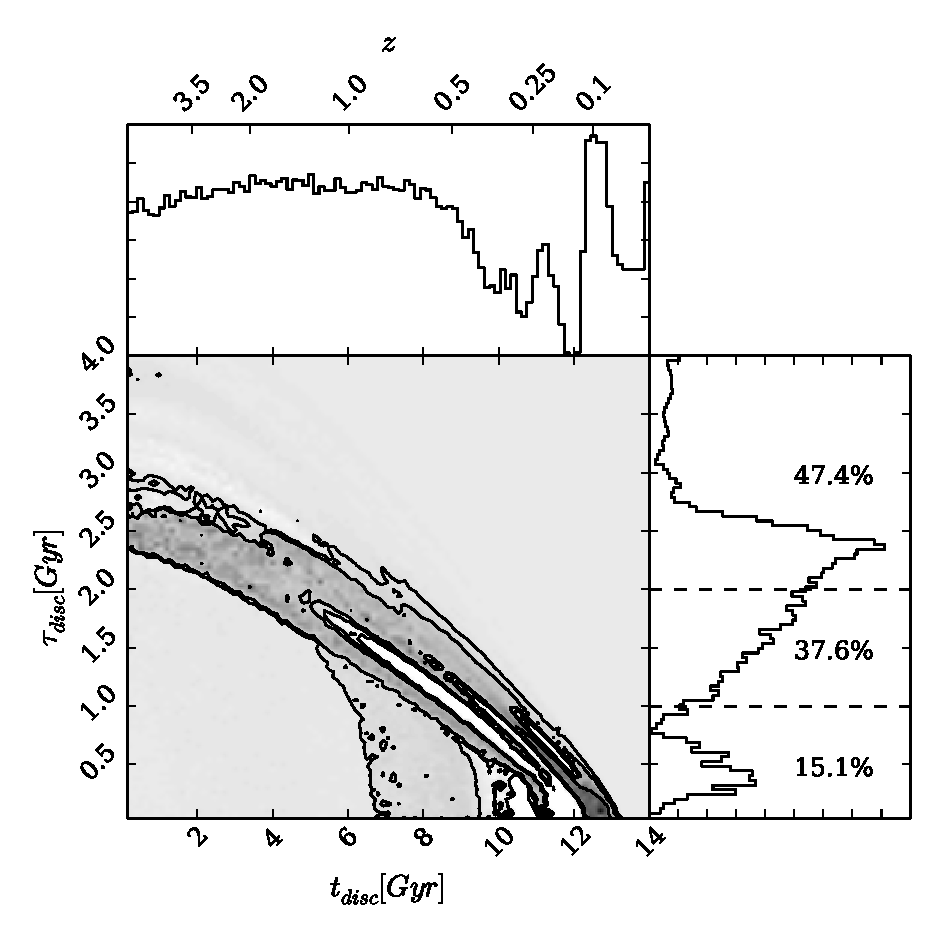
\includegraphics[width=0.4975\textwidth]{green_disc.pdf}
\caption{Contour plots showing the summed posterior probability distribution function weighted by the morphological vote fractions from GZ2 to give the areas of high likelihood in the model parameter space for both elliptical (left) and disc (right) dominated systems. The histograms show the projection into one dimension for each parameter. The dashed lines show the separation between rapid ($\tau ~\rm{[Gyr]} < 1.0$), intermediate ($1.0 < \tau ~\rm{[Gyr]} < 2.0$) and slow ($\tau ~\rm{[Gyr]} > 2.0$) quenching timescales with the fraction of the combined posterior probability distribution in each region shown}.

\label{green_v}
\end{figure*}

The SFH models were implemented with the \starpy ~package to produce Figures~\ref{red_s} \&\ref{green_v} for the red sequence, green valley and blue cloud populations of smooth and disc galaxies respectively. The percentages shown in Figures~\ref{red_s} \& \ref{green_v} are calculated as the fractions of the combined posterior probability distribution located in each region of parameter space for a given population. 

The left panel of Figure~\ref{red_s} reveals that smooth galaxies with red optical colours show a preference $(49.5\%$; see Figure~\ref{red_s}) for rapid quenching timescales across all cosmic time. For these smooth red galaxies we see, at early times only, a preference for slow and intermediate timescales. The right panel of Figure~\ref{red_s} reveals that red disc galaxies show are dominated by slow $(44.1\%)$ quenching timescales. The preference for \emph{very} slow ($\tau > 3.0 ~\rm{Gyr}$) quenching timescales (which are not seen for the green valley discs) suggests that these galaxies have only just reached the red sequence after a very slow evolution across the colour-magnitude diagram.

In Figure~\ref{green_v} intermediate quenching timescales become more significant (in agreement with the conclusions of \citealt{Gonc12}), particularly for smooth-like galaxies (see the left panel of Figure~\ref{green_v}).

The smooth galaxy parameters favour these intermediate quenching timescales ($40.6\%$) with some preference for slow quenching at  early times ($z > 1$). The preference for rapid quenching of smooth galaxies has dropped by over a half compared to the red galaxies.The disc galaxies of the green valley now overwhelmingly prefer slow quenching timescales ($47.4\%$). If we compare Figure~\ref{green_v} to Figure~\ref{red_s} we can see quenching has occurred at later (more recent) cosmic times in the green valley for both morphological types. Therefore both morphologies are tracing the evolution of the red sequence.

In summary, rapid quenching is much more prevalent in smooth galaxies than disc galaxies, and the red galaxies  are also much more likely to be characterised by a rapid quenching model than green valley galaxies. In the green valley there is also a distinct lack of preference for rapid quenching timescales with $\tau < 0.5~\rm{Gyr}$, more so for the disc- than the smooth-like galaxies. This suggests that this rapid quenching mechanism causes a change in morphology from a disc- to a smooth-like galaxy as a galaxy moves across the colour magnitude diagram.

One simulation of interest by \citet{Springel05} showed that feedback from black hole activity is a necessary component of destructive major mergers to produce such rapid quenching timescales. They find using hydrodynamical simulations that after $\sim1~\rm{Gyr}$ the merger remnant has reddened to $u-r \sim 2.0$. This is in agreement with my simple quenching models which give that within $\sim1~\rm{Gyr}$ the models with a SFH with $\tau < 0.4~\rm{Gyr}$ have reached the red sequence with $u-r ~\ga 2.2$. In comparison the simulations of \citet{Springel05} without any feedback from black holes, suggest that if even a small fraction of gas is not consumed in the starburst following a merger (either because the mass ratio is not large enough or from the lack of strong black hole activity) the remnant can sustain star formation for periods of several Gyrs. The remnants from these simulations take $\sim5.5~\rm{Gyr}$ to reach red optical colours of $u-r \sim 2.1$. This is again in agreement with my simple quenching models with intermediate quenching timescales of $1.0 \la ~\tau~\rm{[Gyr]} ~\la 2.0$ which take approximately $2.5-5.5~\rm{Gyr}$ to reach these red colours.

These intermediate quenching timescales are found to be equally prevalent across populations for both smooth and disc galaxies across cosmic time particularly in the green valley. Intermediate timescales are the prevalent mechanism for quenching smooth green valley galaxies, unlike the rapid quenching prevalent for red galaxies. We suggest that this intermediate quenching route must therefore be possible with routes that both preserve and transform morphology. It is this result of another route through the green valley that is in contradiction with the findings of \cite{Sch2014}. 

\begin{figure*}
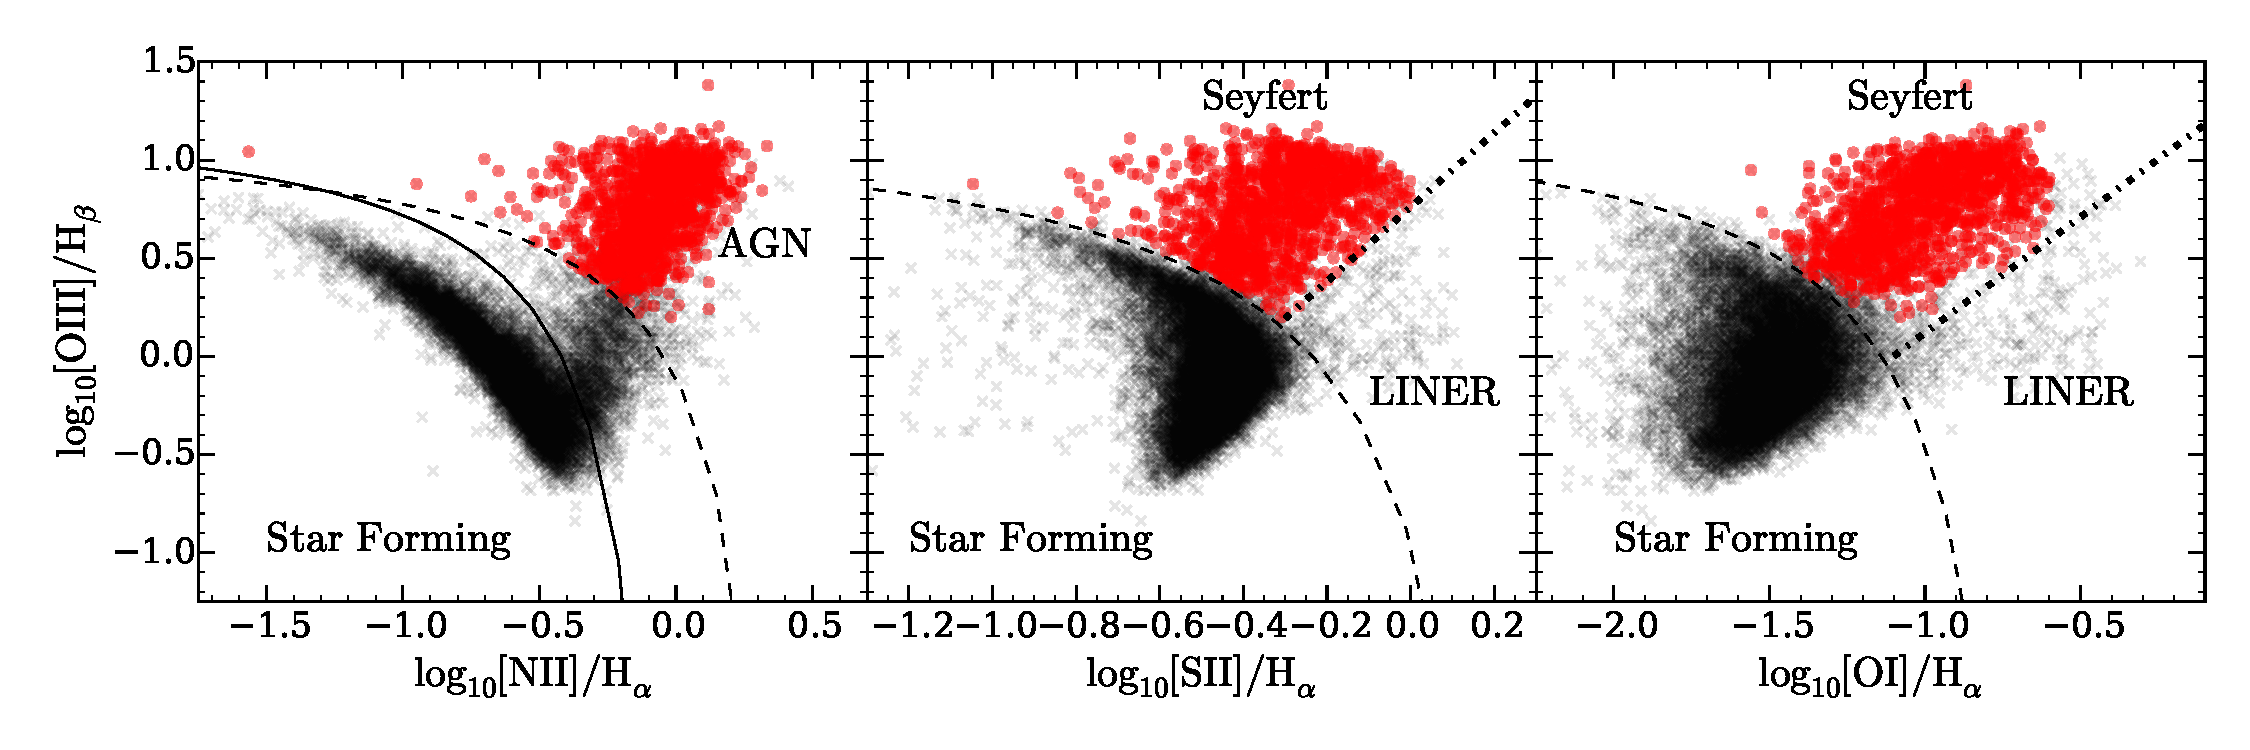
\includegraphics[width=0.94\textwidth]{GZ2_GALEX_sample_bpt_diagram_SNR_gtr_3_type_1_seyferts_only_better_quality.pdf}
\caption{BPT diagrams for galaxies in the \textsc{gz2-galex} sample (black crosses) with S/N $> 3$ for each emission line. Inequalities defined in: \cite{Kew01} to separate SF galaxies from AGN (dashed lines), \cite{Kauff03b} to separate SF from composite SF-AGN galaxies (solid line) and \cite{Kew06} to separate LINERS and Seyferts (dotted lines). Galaxies are included in the \textsc{agn-host} sample (red circles) if they satisfy all the inequalities to be classified as Seyferts.}
\label{bpt}
\end{figure*}

We speculate that the intermediate quenching timescales are caused by gas rich major mergers, major mergers without black hole feedback and from minor mergers, the latter of which is the dominant mechanism.

Although intermediate and rapid quenching timescales are the dominant mechanisms across the colour-magnitude diagram, together they cannot completely account for the quenching of disc galaxies. There is also a significantly lower preference for smooth galaxies to undergo such slow quenching timescales; suggesting that the evolution (or indeed creation) of typical smooth galaxies is dominated by processes external to the galaxy. 

\citet{Bamford09} using GZ1 vote fractions of galaxies in the SDSS, found a significant fraction of high stellar mass red spiral galaxies in the field. As these galaxies are isolated from the effects of interactions from other galaxies, the slow quenching mechanisms present in their preferred star formation histories are most likely due to secular processes (i.e. mechanisms internal to the galaxy, in the absence of sudden accretion or merger events; \citealt{KK04, Sheth12}). Bar formation in a disc galaxy is such a mechanism, whereby gas is funnelled to the centre of the galaxy by the bar over long timescales where it is used for star formation \citep{Masters12, Saint12, Cheung13}, consequently forming a `pseudo-bulge' \citep{Kormendy10, Simmons13}.

If we believe that these slow quenching timescales are due to secular evolution processes, this is to be expected since these processes do not change the disc dominated nature of a galaxy. 


\subsection{Type 2 AGN Host Quenching Histories}\label{agn}

The prevalence of rapid quenching rates found for smooth-like galaxies in the red sequence and their connection to black hole activity discussed above led to an investigation of the star formation histories across a population of Type 2 AGN host galaxies. Type 2 AGN were used to investigated this connection due to their photometric obscuration and were selected using a BPT diagram \citep{bpt81} using line and continuum strengths for [OIII], [NII], [SII] and [OII] obtained from the MPA-JHU catalogue \citep{Kauff03, Brinch04} for the galaxies studied above. We then required the S/N $> 3$ for each emission line as in \cite{Sch2010}. Those galaxies which satisfied all of the inequalities defined in \cite{Kew01} and \cite{Kauff03b} to be classified as Seyfert galaxies were selected giving $1,244$ AGN host galaxies and are shown in red in Figure \ref{bpt}. LINERs (shown not to be primarily powered by AGN) and composite galaxies were removed for purity. We refer to this sample as the \textsc{agn-host} sample.

We constructed a sample of inactive galaxies by removing from the \textsc{gz2-galex} sample all galaxies in the \textsc{agn-host} sample, as well as sources identified as Type 1 AGN by the presence of broad emission lines \citep{Oh15}. We refer to this sample as the \textsc{inactive} sample. 

We also split both the \textsc{agn-host} and \textsc{inactive} samples into low, medium and high mass ranges (see Figures \ref{time} \& \ref{rate} to investigate any trends in the SFH with mass. Masses were calculated using the $(u-r)$ colour and absolute $r$-band magnitude with the method outlined in \cite{Baldry06}.

We apply the method outlined in Section \ref{starpy} to obtain a 2-dimensional likelihood distribution across the $[t_q, \tau]$ parameter space. We combine individual galaxy likelihood distributions within the \textsc{agn-host} and \textsc{inactive} galaxy samples, additionally weighting by GZ2 morphologies to produce quenching parameter likelihood distributions for both disc- and smooth-dominated galaxy populations as in section \ref{gv}. In Figures \ref{time} and \ref{rate} we show only the one dimensional histograms across each parameter. 


\begin{figure}
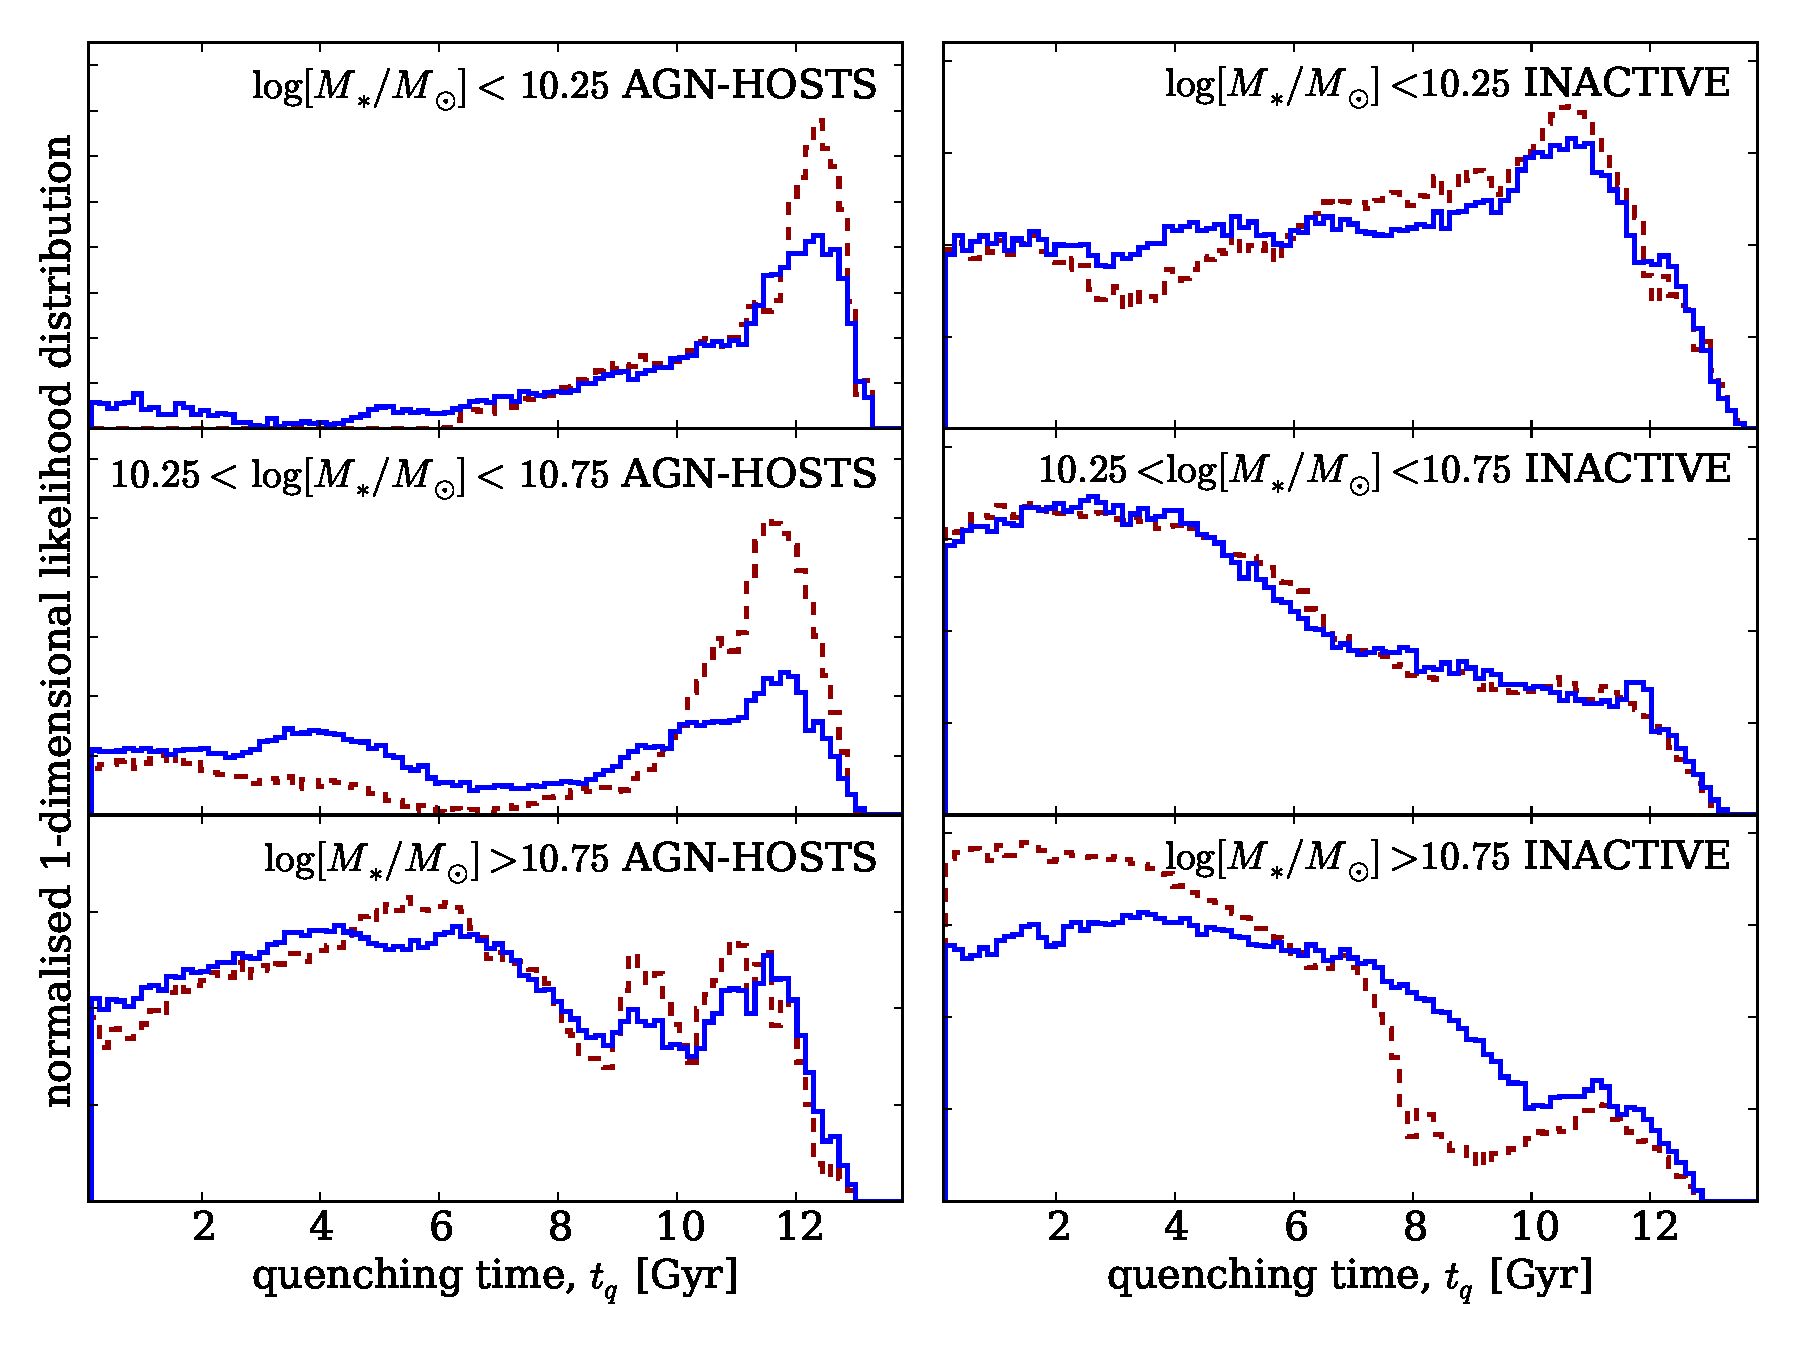
\includegraphics[width=0.485\textwidth]{quenching_time_histograms_smooth_red_disc_blue_verticalbpt_seyf_only_hardcut_minimal.pdf}
\caption{Likehood distribution for the quenching time, $t_q$ parameter normalised so that the areas under the curves are equal. \textsc{agn-host} (left) and \textsc{inactive} (right) galaxies are split into low (top), medium (middle) and high (bottom) mass for smooth (red dashed) and disc (blue solid) galaxies. A low value of $t_q$ corresponds to the early Universe and a high value to the recent Universe.}
\label{time}
\end{figure}

\begin{figure}
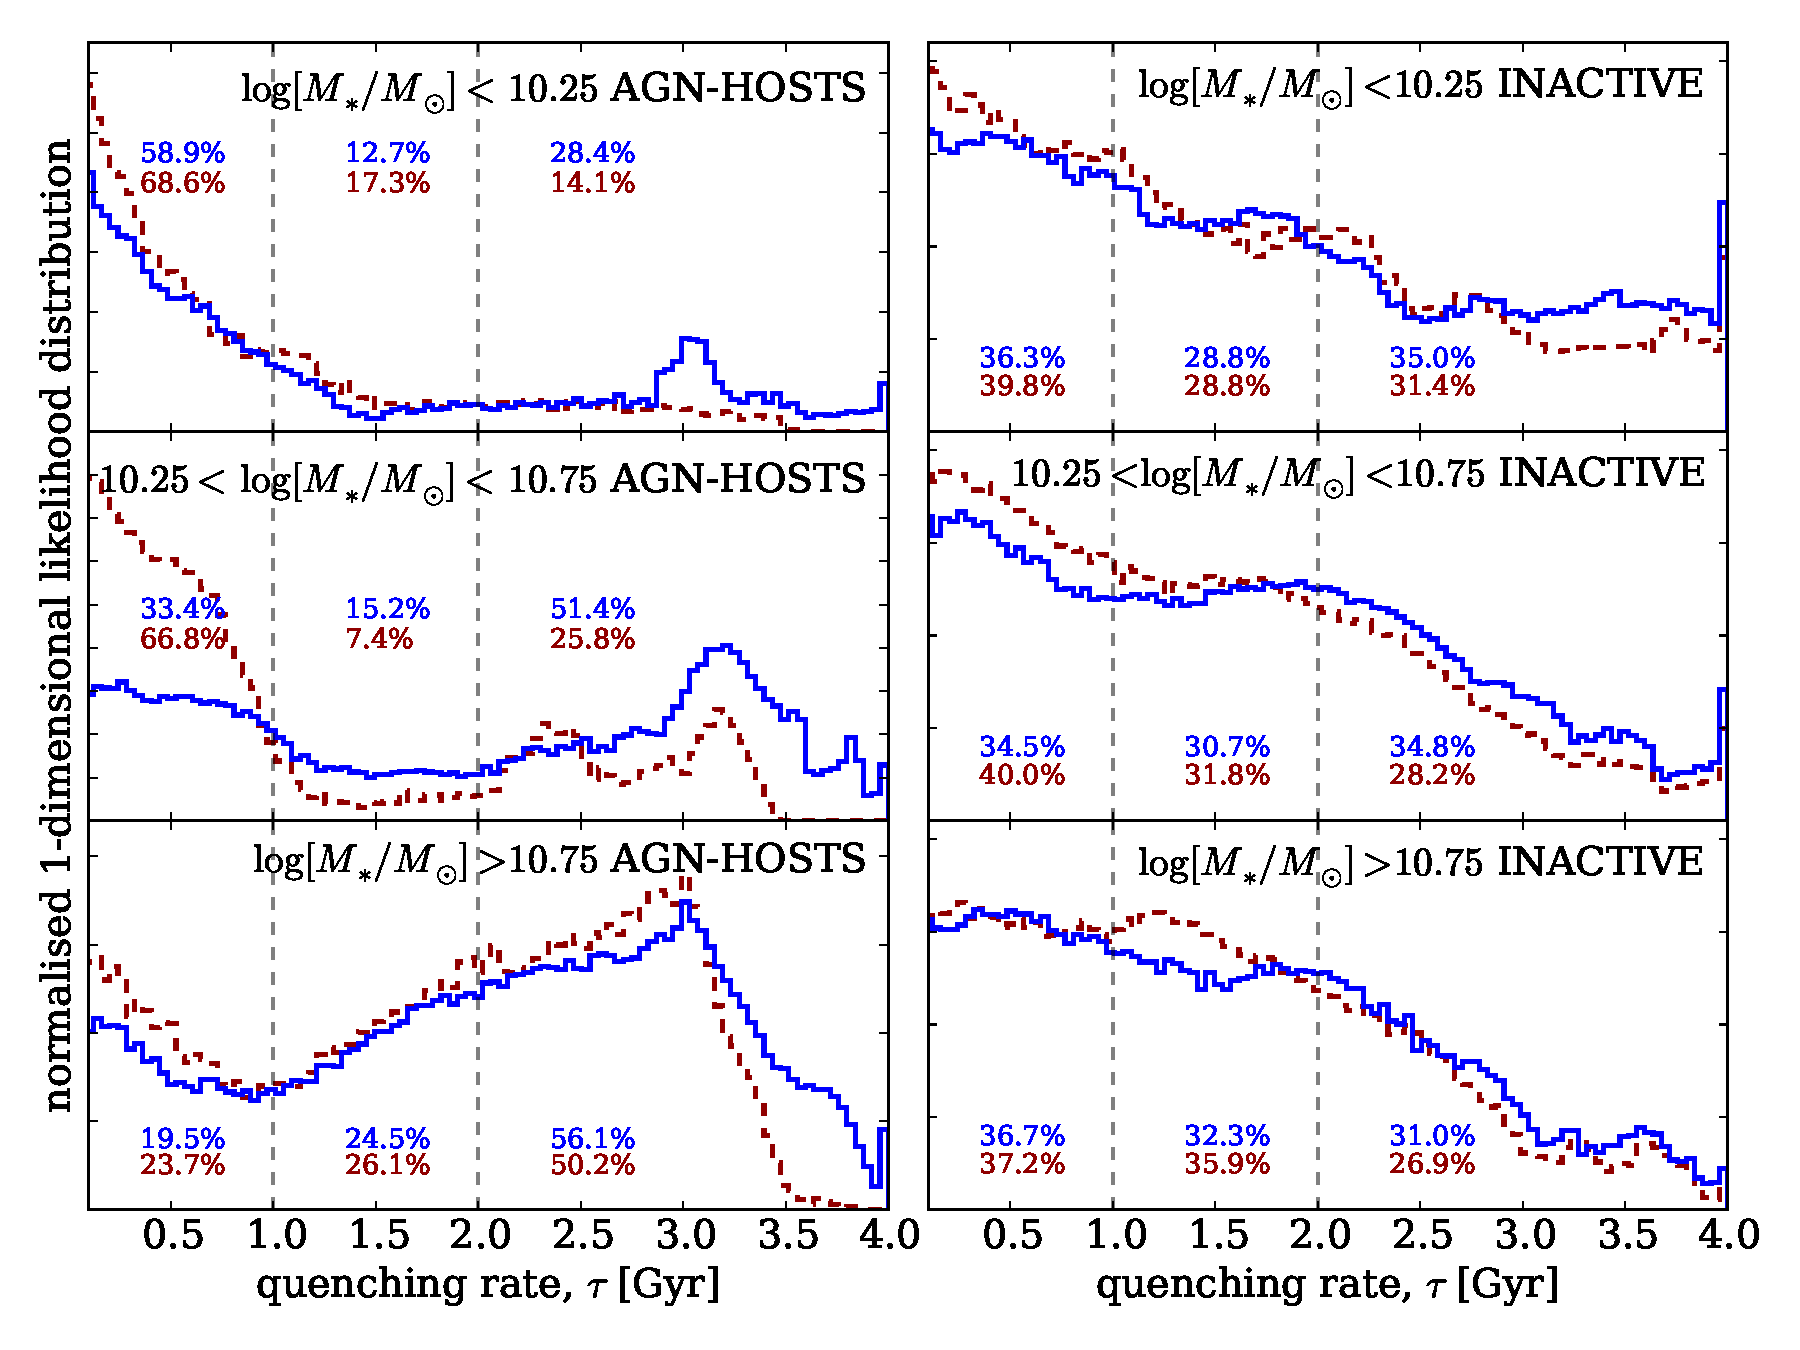
\includegraphics[width=0.485\textwidth]{quenching_rate_histograms_smooth_red_disc_blue_verticalbpt_seyf_only_hardcut_minimal.pdf}
\caption{Likehood distribution for the quenching rate, $\tau$ normalised so that the areas under the curves are equal. \textsc{agn-host} (left) host and \textsc{inactive} (right) galaxies are split into low (top), medium (middle) and high (bottom) mass for smooth (red dashed) and disc (blue solid) galaxies. The black dashed lines show the separation between rapid ($\tau < 1.0$ Gyr), intermediate ($1.0 < \tau ~\rm{[Gyr]} < 2.0$) and slow ($\tau > 2.0$ Gyr) quenching timescales with the percentage likelihood distribution in each region for disc (blue) and smooth (red) populations. A small (large) value of $\tau$ corresponds to a rapid (slow) quench.}
\label{rate}
\end{figure}


At all masses, the distribution of likelihood for the \textsc{agn-host} population across the quenching time $t_q$ parameter (left panels of Figure \ref{time}) is different from that of the inactive galaxies (right panels of Figure \ref{time}). Recent quenching ($t > 11$ Gyr) of \textsc{agn-host} galaxies is the dominant history for low and medium mass galaxies, particularly for the smooth galaxy population. However, this effect is less dominant in higher mass galaxies where quenching at earlier times has significant likelihood.

The distributions of likelihood for the quenching rate, $\tau$, in Figure \ref{rate} show the dominance of rapid quenching ($\tau < 1$ Gyr) across the \textsc{agn-host} population, particularly for smooth galaxies. With increasing mass the dominant quenching rate becomes slow ($\tau > 2$ Gyr) especially for disc galaxies hosting an AGN. Similar trends in likelihood are observed for the \textsc{inactive} population but the overall distribution of likelihood is very different. 

The likelihood distribution for the \textsc{agn-host} galaxies therefore shows evidence for the dominance of rapid, recent quenching having occurred across the entire population. This result implies the importance of AGN feedback for the evolution of these galaxies.

\cite{Torbra09} model the effects of negative AGN feedback on a typical early type (i.e. smooth) galaxy and find the time between the current galaxy age in their simulation, $t_{gal}$ and the time that the feedback began, $t_{AGN}$, peaks at $t_{gal} - t_{AGN} \sim 0.85 ~\rm{Gyr}$. This agrees with the location of the peak in Figure \ref{time} for low mass galaxies, where the difference between the peak of the likelihood and the average age of the population (galaxy age is calculated from the redshift by assuming all galaxies form at $t=0$) is $\sim0.83 ~\rm{Gyr}$. This implies that this dominant recent quenching history is caused directly by AGN feedback, as opposed to the AGN being a consequence of an alternative quenching mechanism.

Rapid quenching is particularly dominant for low-to-medium mass smooth galaxies. \cite{Sme2015} suggest that incredibly rapid quenching rates could be attributed to mergers of galaxies in conjunction with AGN feedback, which are thought to be responsible for creating the most massive smooth galaxies \citep{Con03, Springel05, Hopkins08}. This dominance of rapid quenching across the smooth \textsc{agn-host} population supports the idea that a merger, having caused a morphological transformation to a smooth galaxy, can also trigger an AGN, causing feedback and cessation of star formation (see Figure 14 of \citealt{Sch2014}).


\section{Thesis Development}\label{plan}
The two main results discussed above in Sections \ref{gv} \& \ref{agn} will form the basis of my thesis with an in depth discussion of the limitations of \starpy and the uncertainties associated with it. I am also currently investigated the connection between the morphology and the cluster environment of galaxies in the \textsc{gz2-galex} sample, the results of which I hope will populate another chapter. 

A plan for my thesis is highlighted below with two line abstracts for each chapter. 

\begin{enumerate}[I]
\item{{\bf Introduction}: The morphological evolution of galaxies across the colour magnitude diagram is intrinsically tied to the quenching of star formation. There has been much speculation on the possible processes driving this evolution.}

\item{{\bf Galaxy Zoo}: Galaxy Zoo is a citizen science project which asks users to classify the morphology of SDSS images of galaxies using a simple web interface. The output from this project is statistically robust, reliable morphological classifications for 250,000+ galaxies.}

\item{{\bf STARPY~}: \starpy~ is a piece of software which allows the user to determine the likelihood distribution for the 2D star formation history of a galaxy given two photometric colour measurements and a redshift. This is determined using Bayesian statistics and Markov Chain Monte Carlo methods to produce robust statistical results.}

\item{{\bf Quenching across the Colour Magnitude Diagram}: Green valley galaxies are thought to be the evolutionary missing link between the red sequence of red, dead, massive galaxies and the blue cloud of blue, star forming, less massive galaxies. Recent work showed highlighted radically different pathways of quenching for different morphological types, here I show, using \starpy~, that diverse quenching mechanisms with a large range of quenching rates are instrumental in forming the present day red sequence.}

\item{{\bf Type 2 AGN Host Quenching Histories}: The co-evolution of galaxies and their central super massive black holes has long been theorised with ideas of negative feedback from AGN causing quenching in galaxies. Using \starpy~ I demonstrate that a population of Type 2 AGN galaxies shows a strong likelihood for rapid quenching occurring in the last 2 Gyr which is not found for a population of currently inactive galaxies.}

\item{{\bf Environmental Quenching Dependancies}: The density in which a galaxy evolves has a significant effect on the morphology of a galaxy by either restricting, providing or rationing the gas available for star formation. Using \starpy~ I (hope to) demonstrate how the rate of quenching is dependent on a galaxies position in a cluster as either a central or satellite.}

\item{{\bf Observational Evidence}: Observing runs were completed at the Isaac Newton Telescope, La Palma, Canary Islands and at the Caltech Submillimeter Observatory, Hawaii. Observations of both bulgeless galaxies with growing black holes and blue elliptical galaxies were taken as observational support of the theories discussed in support of the research findings above.} 

\item{{\bf Discussion \& Conclusion}: There is a clear difference between the quenching timescales of smooth and disc dominated galaxies suggesting that the processes driving quenching are morphologically dependant. However, whether the properties of galaxies observed (e.g. the presence of an AGN, tidal tails, location in cluster etc.) are the cause or consequence of these quenching mechanisms is still under discussion here.}
\end{enumerate}


\section{Conclusion}
I have used morphological classifications from the Galaxy Zoo 2 project to determine the morphology-dependent star formation histories across the colour magnitude diagram and in a population of AGN host galaxies. We determined the most likely parameters for the quenching onset time, $t_q$, and exponential quenching rate, $\tau$, and find clear differences in the combined population likelihoods between red sequence and green valley galaxies, providing evidence for the possible driving mechanisms behind this quenching including secular evolution, galaxy interactions and mergers with and without AGN. the  inactive and AGN host galaxy populations. In particular this relationship between the quenched star formation histories and the presence of a type 2 AGN has been shown with evidence that a population of AGN host galaxies having recently undergone a rapid drop in their star formation rate. This result provides strong observational support for AGN feedback in these systems, but this work also shows that feedback cannot be responsible for all of the quenching across the AGN host population


\begin{thebibliography}{}
\bibitem[\protect\citeauthoryear{Baldry et al.}{2004}]{Baldry04} Baldry, I. K. et al., 2004, ApJ, 600, 681
\bibitem[\protect\citeauthoryear{Baldry et al.}{2006}]{Baldry06} Baldry, I. K. et al., 2006, MNRAS, 373, 469
\bibitem[\protect\citeauthoryear{Baldwin, Phillips \& Terlevich}{1981}]{bpt81} Baldwin, J. A., Phillips, M. M., \& Terlevich, R. 1981, PASP, 93, 5
\bibitem[\protect\citeauthoryear{Ball, Loveday \& Brunner}{2008}]{BLB08} Ball, N. M., Loveday, J. \& Brunner, R. J., 2008, MNRAS, 383, 907
\bibitem[\protect\citeauthoryear{Bamford et al.}{2009}]{Bamford09} Bamford, S. P. et al., 2009, MNRAS, 393, 1324
\bibitem[\protect\citeauthoryear{Brammer et al.}{2009}]{Brammer09} Brammer, G. B. et al., 2009, ApJ, 706, 173
\bibitem[\protect\citeauthoryear{Brinchmann et al.}{2004}]{Brinch04} Brinchmann, J. et al., 2004, MNRAS, 351, 1151

\bibitem[\protect\citeauthoryear{Bruzual \& Charlot}{2003}]{BC03} Bruzual, G. \& Charlot, S., 2003, MNRAS, 344, 1000
\bibitem[\protect\citeauthoryear{Cheung et al.}{2013}]{Cheung13} Cheung, E. et al., 2013, ApJ, 779, 162
\bibitem[\protect\citeauthoryear{Conselice et al.}{2003}]{Con03} Conselice, C. J. et al., 2003, AJ, 126, 1183
\bibitem[\protect\citeauthoryear{Darg et al.}{2010}]{Darg10a} Darg, D. et al., 2010a, MNRAS, 401, 1552
\bibitem[\protect\citeauthoryear{Faber et al.}{2007}]{Faber07} Faber, S. M. et al., 2007, ApJ, 665, 265
\bibitem[\protect\citeauthoryear{Foreman-Mackey et al.}{2013}]{Dan} Foreman-Mackey, D., Hogg, D. W., Lang, D., Goodman, J., 2013, PASP, 125, 306
\bibitem[\protect\citeauthoryear{Gon\c calves et al.}{2012}]{Gonc12} Gon\c calves, T. S. et al., 2012, ApJ, 759, 67
\bibitem[\protect\citeauthoryear{Hasinger}{2008}]{Hasinger08} Hasinger, G., 2008, A\&A, 490, 905
\bibitem[\protect\citeauthoryear{Hopkins et al.}{2008}]{Hopkins08} Hopkins, F. et al., 2008, ApJSS, 175, 390

\bibitem[\protect\citeauthoryear{Kauffman et al.}{2003a}]{Kauff03} Kauffman, G. et al., 2003, MNRAS, 341, 33
\bibitem[\protect\citeauthoryear{Kauffman et al.}{2003b}]{Kauff03b} Kauffman, G. et al., 2003, MNRAS, 346, 1055
\bibitem[\protect\citeauthoryear{Kewley et al.}{2001}]{Kew01} Kewley, L. J. et al., 2001, ApJ, 556, 121
\bibitem[\protect\citeauthoryear{Kewley et al.}{2006}]{Kew06} Kewley, L. J. et al., 2006, MNRAS, 372, 961
\bibitem[\protect\citeauthoryear{Kormendy \& Kennicutt}{2004}]{KK04} Kormendy, J. \& Kennicutt, R. J., 2004, ARA\&A, 42, 603
\bibitem[\protect\citeauthoryear{Kormendy et al.}{2010}]{Kormendy10} Kormendy, J. et al., 2010, ApJ, 723, 54
\bibitem[\protect\citeauthoryear{MacKay}{2003}]{MacKay} MacKay, D. J. C., 2003, \emph{Information Theory, Inference and Learning Algorithms}, Cambridge University Press, ISBN 978-0-521-64298-9
\bibitem[\protect\citeauthoryear{Marasco, Fraternali \& Binney}{2012}]{MFB12} Marasco, A., Fraternali, F. \& Binney, J. J., 2012, MNRAS, 419, 1107
\bibitem[\protect\citeauthoryear{Martin et al.}{2007}]{Martin07} Martin, D. C. et al., 2007, ApJS, 173, 342
\bibitem[\protect\citeauthoryear{Masters et al.}{2010a}]{Masters10} Masters, K. L. et al., 2010, MNRAS, 405, 783
\bibitem[\protect\citeauthoryear{Masters et al.}{2011}]{Masters11} Masters, K. L. et al., 2011, MNRAS, 411, 2026
\bibitem[\protect\citeauthoryear{Masters et al.}{2012}]{Masters12} Masters, K. L. et al., 2012, MNRAS, 424, 2180
\bibitem[\protect\citeauthoryear{Mendez et al.}{2011}]{Mendez11} Mendez, A. J. et al., 2011, ApJ, 736, 110
\bibitem[\protect\citeauthoryear{Nandra et al.}{2007}]{Nandra07} Nandra, K. et al., 2007, ApJ, 660, L11
\bibitem[\protect\citeauthoryear{Noeske et al.}{2007}]{Noeske07} Noeske, K. G. et al., 2007, ApJ, 660, L43
\bibitem[\protect\citeauthoryear{Oh et al.}{2015}]{Oh15} Oh, K. et al. 2015, arXiv: 1504.07247
\bibitem[\protect\citeauthoryear{Peng et al.}{2010}]{Peng} Peng, Y. et al., 2010, ApJ, 721, 193
\bibitem[\protect\citeauthoryear{Saintonge et al.}{2012}]{Saint12} Saintonge, A. et al., 2012, ApJ, 758, 73
\bibitem[\protect\citeauthoryear{Salim et al.}{2007}]{Salim07} Salim, S. et al., 2007, ApJSS, 173, 267
\bibitem[\protect\citeauthoryear{Schawinski et al.}{2007}]{Sch07} Schawinski, et al., 2007, MNRAS, 382, 1415
\bibitem[\protect\citeauthoryear{Schawinski et al.}{2010}]{Sch2010} Schawinski, K. et al., 2010, MNRAS, 711, 284
\bibitem[\protect\citeauthoryear{Schawinski et al.}{2014}]{Sch2014} Schawinski, K. et al., 2014, MNRAS, 440, 889
\bibitem[\protect\citeauthoryear{Sheth et al.}{2012}]{Sheth12} Sheth, K. et al., 2012, ApJ, 758, 136

\bibitem[\protect\citeauthoryear{Silverman et al.}{2008}]{Silverman08} Silverman, J. D., et al. 2008, ApJ, 675, 1025
\bibitem[\protect\citeauthoryear{Simmons et al.}{2013}]{Simmons13} Simmons, B. D. et al., 2013, MNRAS, 429, 2199
\bibitem[\protect\citeauthoryear{Sivia}{1996}]{Sivia} Sivia, D. S., 1996, \emph{Data Analysis: A Bayesian Tutorial}, Oxford University Press, ISBN 0-19-851889-7
\bibitem[\protect\citeauthoryear{Springel, Di~Matteo \& Hernquist}{2005}]{Springel05} Springel, V., Di Matteo, T. \& Hernquist, L., 2005, ApJ, 620, L79
\bibitem[\protect\citeauthoryear{Smethurst et al.}{2015}]{Sme2015} Smethurst, R. J. et al., 2015, MNRAS, 450, 435
\bibitem[\protect\citeauthoryear{Tortora et al.}{2009}]{Torbra09} Tortora, C. et al., 2009, MNRAS, 369, 61
\bibitem[\protect\citeauthoryear{Willett et al.}{2013}]{GZ2} Willett, K. et al., 2014, MNRAS, 435, 2835
\bibitem[\protect\citeauthoryear{Willmer et al.}{2006}]{Willmer06} Willmer, C. N. A. et al., 2006, ApJ, 647, 853
\end{thebibliography}

\end{document}
